\section{Methodology}

\begin{figure*}[t!]
\centering
\includegraphics[width=\textwidth]{./New_prisma_chart.png}
\caption{Prisma chart}
\label{fig1}
\end{figure*}

\begin{figure*}[h!]
\centering
\includegraphics[width=\textwidth]{./bibliometricalanalysis.png}
\caption{Bibliometrical analysis. a) shows the growing annual number of publications, b) the share of journals and publishing houses, c) the world map of countries with the most papers, and d) the journals with the most papers}
\label{bibliometrical}
\end{figure*}

We follow the PRISMA convention for reporting the search and selection
process of scientific studies in systematic reviews, as shown in Fig.
\ref{fig1}.

We conducted the search and mass extraction of articles from the Scopus
database using advanced Search in the fields title, abstract and
keywords. The search covered the period 2016--2026, was restricted to
English-language documents, and included the document types article,
review and conference paper. The subject areas included energy,
engineering and computer science. The search was exported on 2026-05-05
and returned 3129 records. The following search query was used:

> (\"surrogate model\" OR \"surrogate models\" OR \"surrogate modeling\"
> OR\
> \"surrogate modelling\" OR \"surrogate assisted\" OR metamodel\* OR\
> metamodeling OR metamodelling OR emulator OR emulators OR emulation
> OR\
> \"response surface\" OR kriging OR \"gaussian process\" OR\
> \"polynomial chaos\" OR \"radial basis function\" OR\
> \"support vector regression\" OR \"random forest\" OR \"gradient
> boosting\" OR\
> \"neural network proxy\" OR \"machine learning surrogate\" OR\
> \"data driven surrogate\" OR \"neural surrogate\" OR \"learning to
> optimize\" OR\
> \"optimization proxy\" OR \"optimization proxies\")\
> AND\
> (\"energy system\" OR \"power system\" OR \"electricity system\" OR\
> \"electric power system\" OR \"district heating\" OR \"district
> energy\" OR\
> \"multi energy\" OR \"multi energy system\" OR \"integrated energy
> system\" OR\
> \"sector coupling\" OR \"sector coupled\" OR \"unit commitment\" OR\
> \"economic dispatch\" OR \"optimal power flow\" OR \"capacity
> expansion\" OR\
> \"generation expansion\" OR \"energy planning\" OR \"energy dispatch\"
> OR\
> \"energy scheduling\" OR microgrid\* OR \"smart grid\" OR\
> \"renewable energy system\" OR \"power grid\")\
> AND\
> (optimization OR optimisation OR dispatch OR scheduling OR planning
> OR\
> \"stochastic programming\" OR \"robust optimization\" OR \"chance
> constraint\" OR\
> \"multi objective\" OR pareto OR milp OR \"mixed integer\" OR bilevel
> OR\
> \"scenario reduction\")

\begin{figure}[t!]
\centering
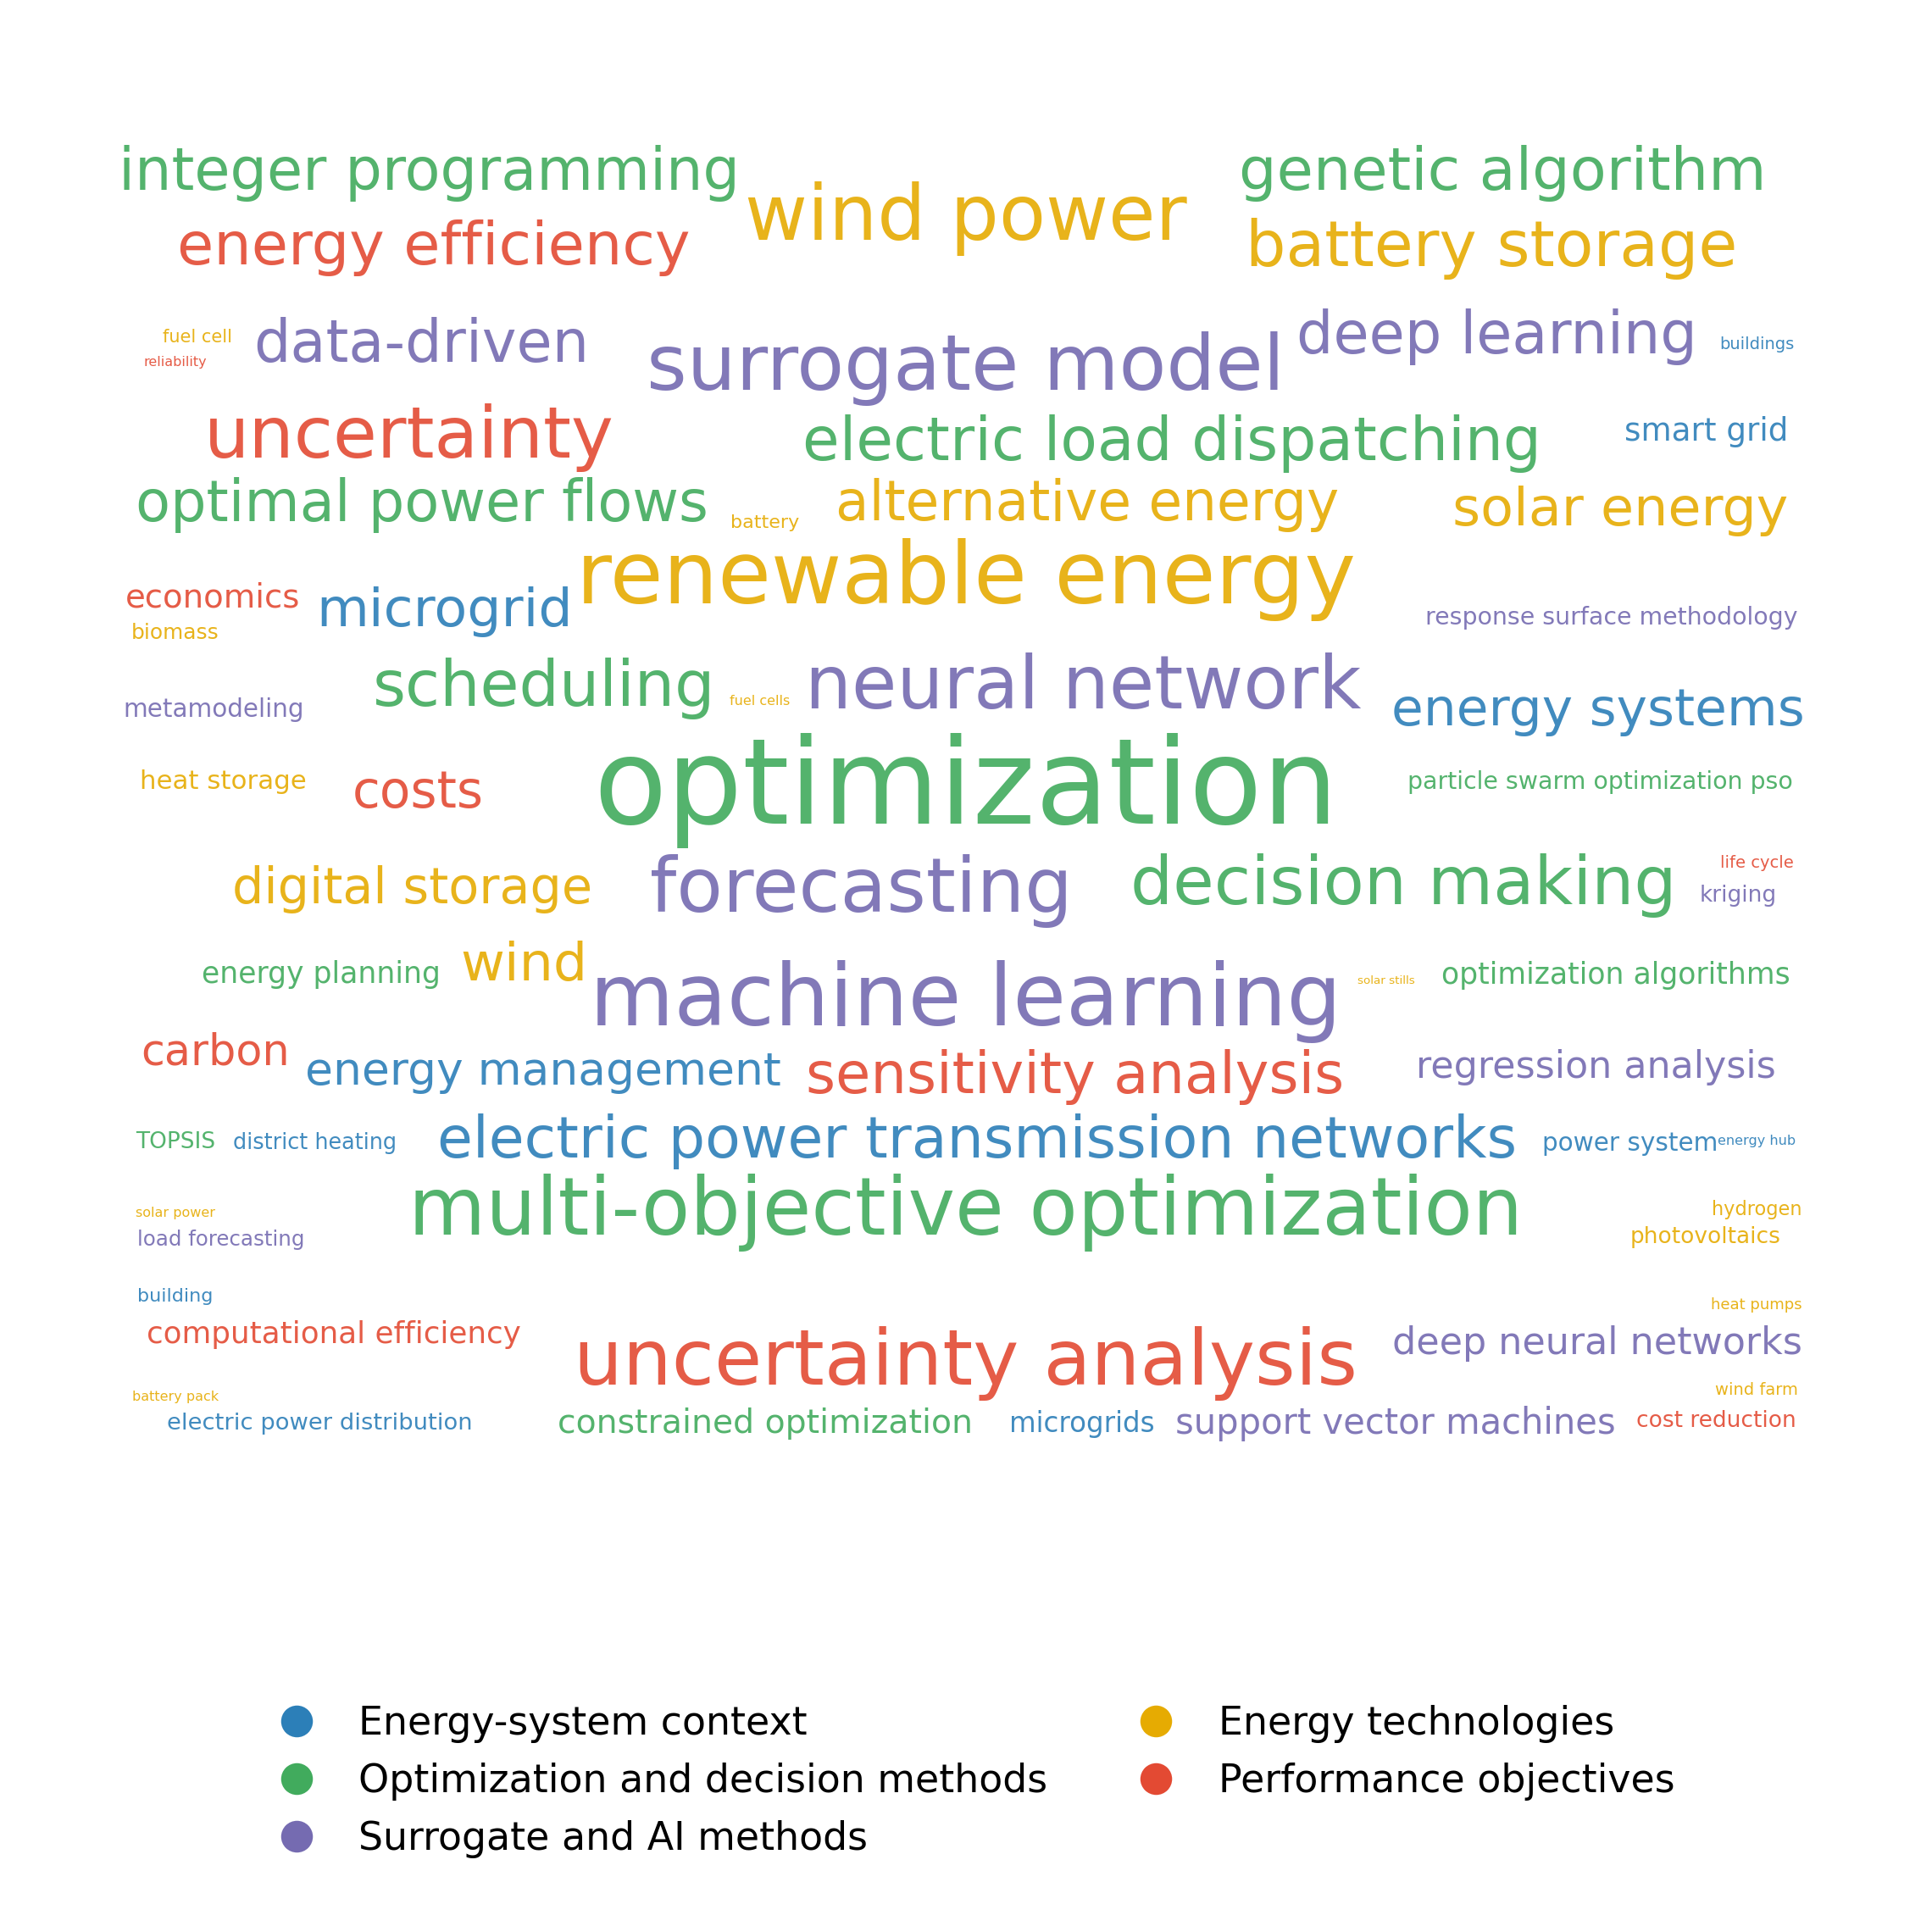
\includegraphics[width=0.98\\linewidth]{../figures/fig_bibliometric_keyword_wordcloud.png}
\caption{Keywords}
\label{fig1}
\end{figure}

For each exported citation record, title, abstract and keywords were
merged into a single text field and classified using a rule-based
screening process. Records were included when explicitly containing
surrogate or metamodel vocabulary, such as surrogate, metamodel,
kriging, Gaussian process, polynomial chaos, response surface or
learning to optimize, with a clear reference to energy systems. These
records were accepted as core literature on surrogate modeling in
optimization-related energy system modeling (n = 1270).

Records which did not contain the explicit surrogate/metamodel
vocabulary mentioned above but showed (i) machine-learning or regression
methodology, (ii) an optimization focus, (iii) an energy-system focus,
and (iv) at least one reference to replacement, approximation or
computation-time reduction compared to an expensive original model were
marked for manual review before included in the main body of analyzed
records (n = 154). A small additional subset (n = 4) was marked as
likely out of scope, because strong non-target signals, such as pure
error diagnosis or site selection without an optimization surrogate. All
remaining records were classified as out of scope (n = 1701), because
they did not meet the surrogate-for-optimization criteria for further
analysis.

To ensure that the review did not only capture explicitly labelled
surrogate studies, the surrogate-focused export was complemented with
MOO/MES studies, comprising records with a multi-objective or
multicriteria focus and a multi-energy or related system context (n =
1674). Together with the surrogate records, this resulted in 2944
bibliographic records before deduplication. DOI- and key-based
deduplication removed 38 duplicates, yielding a database of 2906
records.

For the manuscript, a subset of 285 studies was selected for further
in-depth analysis. These studies thematically match the narrowed
research focus on surrogate modeling, multi-objectivity, and
multi-energy systems. Moreover, 32 previous reviews or overview articles
including bibliometric reviews, were included in a meta-review based on
title, abstract and keywords and compared with the present article.
